\chapter{INTRODUCTION}
% Følgende informasjon kan tas med her:
% - Organisering av rapporten og kort beskrivelse av sammenhengen mellom kapitlene.
% - Fullstendig definering av oppgaven med utdypning av hva oppgaven går ut på.
% Eksempelvis presiseres mål, problemområde, omfang og avgrensning.
% - Henvisning til eventuelle tidligere arbeider om samme emne.
% - Målgruppe for rapporten, jfr. mål- og mottakeranalysen.
% - Studentenes faglige bakgrunn.
% - Prosjektgruppens valgte arbeidsformer, f.eks. samtaler og intervjuer med kilder, reiser,
% bedriftsbesøk, litteraturstudier, laboratorieforsøk, modellbygging og testing.
% - Terminologibruk. Er eksempelvis faguttrykk brukt i en spesiell betydning?
% Innledningen skal ikke inneholde noe om det som er gjort i oppgaven og oppnådde resultater.


\section{Project Background}
The Norwegian Armed Forces Cyber Defense unit for Computer Network Defense
(CND), Centre for Protection of Critical Infrastructure (Avdeling BKI in
Norwegian), is responsible for detecting and stopping cyber-attacks against the
critical infrastructure and command and control systems utilized by the Norwegian military.
One of the tools used to carry out this task is the open source IDS \snort{}
\cite{Snort}.

\snort{} is a leading \cite{snort_community} open source IDS that is used to
detect potentially unwanted or malicious network traffic based on predefined patterns described in
signatures. There are both free and commercial signatures available for
\snort{} and as \snort{} has been highly adopted by the security community,
these signatures are continually updated and maintained. For large networks, an
IDS will often operate in multiple parts of the network simultaneously, where each separate instance of the IDS is known as a
sensor. 

The management of \snort{} signatures (henceforth referred to as
rules) is cumbersome in multi-sensor environments without a centralized service
which can assure that all sensors are synchronised with the latest rules.
Avdeling BKI has therefore challenged a group of students from Gjøvik University
College (GUC) to design and develop a functional, effective and secure
rule management system for \snort{} that can continue to live on beyond this project.


% Using \snort{} has been plagued for years by the fact that it does not have a good
% system for handling, updating or maintaining the signatures (henceforth called
% rules and rule sets) used for detection, thus making it cumbersome to utilize
% \snort{} for security analysts (ref?).
% 

\section{Previous Work}
Research \cite{BHTB} has shown that a good rule management system for \snort{}
will improve the workflow and efficiency of the IDS significantly, and a
prototype for such a system was built in 2012 called \bringhome{} \cite{BHTB}
(henceforth referred to as \bhtb{}). This prototype has been in use at Avdeling
BKI since 2012, but is suffering from lacks in functionality and efficiency due
to being a proof-of-concept prototype. \bhtb{} has, however, proven that
there is a significant gain from having an intuitive Graphical User Interface
(GUI) for managing rules. A GUI facilitates the work of the operator, as work is
shifted from complex operations in a CLI to automatic execution of common
routines triggered by buttons.

% TODO: improve below paragraph (Eirik)
There was another similar project conducted at \GUC{} in 2012 called
\snortmanager{} \cite{SnortManager} which also deals with management of \snort{}
rules. The \snortmanager{} project files are available as open source
software\cite{snortmanager_repo}, but no usage instructions are available.
The source code has not been maintained since its initial release and is designed for a specific company in mind. Enabling,
disabling and configuring rules is also cumbersome in this system as it is
based on plaintext arguments in ``policies'' that users must construct
themselves \cite{SnortManager}. The rule distribution is also done manually from the
files generated. All this makes \snortmanager{} unsuitable for Avdeling BKI and
their routines.

Several add-ons and other \snort-related software
exist\cite{snort_additional_downloads}, and
a few of these are built to manage \snort{} rules, most notably
\pulledpork{}\cite{pulledpork} and
\oinkmaster{}\cite{oinkmaster}. The key differences
between all software mentioned in this section and \snowman{} will be further
explained in chapter \ref{chap:existing_solutions}.
\section{Project Description}
In broad strokes, the purpose of this project is to design a system
that provides a simple and efficient way of managing rules for the
\snort{} IDS. The project is the spiritual successor to \bhtb{}, and will
essentially expand on the good ideas from \bhtb{}, and add functionality
requested by Avdeling BKI to create a more adoptable open source rule
management system for \snort{}. The project can be broken down into four main
objectives:

\begin{enumerate}
\item Identify the challenges of rule management in IDS's such as \snort{}.
\item Describe how a good rule management system should operate.
\item Develop a good open source rule management system for \snort{}.
\item Measure the performance of the system and compare this to other similar
systems.
\end{enumerate} 
The first two objectives were addressed early on in the project during the
initial design phase of the software. To develop a good rule management system,
it is essential to consider the tasks in the two first objectives, as they form
the basis of how the system in the third objective is designed. Challenges and
best practices in rule management is therefore presented throughout this report
to support the design decisions made in the final software solution.

As the project became very performance-oriented, the report evolved to
also contain a small study into software performance and practical
performance test of related software. 

%tekst flyttet til konklusjon
\section{Target Audence}
\snowman{} is targeted at users of the \snort{} IDS
in a larger production environment with many sensors and networks.
More specifically, the target audience consists of security experts
with a high degree of knowledge of \snort{} and computers in general.

This report is targeted at those which may be interested in discovering just how
complex the rule structure of \snort{} is, and academics that are interested
in reading about IDS software performance testing.

\section{Project objectives}
\label{sec:project_objectives}
\subsection{Result objectives}
As stated in the project plan (Appendix \ref{app:project_plan}), this project
has a goal of researching, designing and developing a system that as a minimum:

\begin{itemize} 
\item Is more efficient than \bhtb{}.
\item Is developed as an engine that responds to API-calls.
\item Is modular in design and allows future changes and additions that will not
affect existing functionality.
\item Is scalable enough to handle both small and large sets of IDS-sensors and
rules in a production environment.
\item Is able to download rules and rulesets from multiple customizable sources.
\item Is able to distribute different rules to different IDS-sensors.
\item Can download and distribute rules automatically at set intervals.
\item Is capable of exporting rules.
\item Has the capability to activate, deactivate, filter and suppress rules on a
per sensor basis, in a user friendly way.
\item Supports multi-user interaction.
\item Can efficiently and safely work with different installations of \snort{} and various
other third party tools, such as SNORBY \cite{snorby}.
\item Is easy to install.
\item Has an internal logging system.
\item Is well-documented and can be easily adopted by anyone as open source
software.
\end{itemize}
In addition, the project group will attempt to add the following functionality:

\begin{itemize}
\item A graphical user interface.
\item The mentioned user interface must be user friendly and intuitive, and
require only limited knowledge of \snort{} rules from the user.
\item The system can also distribute rules to
Suricata \cite{surikata}, another \snort{}-like IDS, which
can operate with the exact same rules as \snort{}.
\item Implement security features that ensure confidentiality of rules.
\item The project will investigate and potentially implement multi-threading
technology or other optimization techniques to exploit modern hardware
capacities.
\item The system is capable of validating and checking rules for errors before
they are distributed to sensors.
\item The system supports commenting of the rules.
\item The system supports writing custom rules and editing existing rules.
\end{itemize}
Once the system is developed, it will be released as an Open Source Software to
the public in a well-documented format.
\subsection{Effect objectives}

Forming baselines from the current prototype \bhtb{} and from \snortmanager{},
the project has a goal to further increase the efficiency of rule management by
investigating and implementing programming techniques such as multi-threading
and caching to reduce latency and delays in the system by as much as 50\%. The
software must also maintain sublinearity in performance, i.e. 10 executions of
the same job should take 10 times, or less, the amount of time as a single
execution.

The achievement of these goals is to be measured by conducting several
performance tests on the final software solution. Results will also be compared
to the performance of \bhtb{} and \snortmanager{}.

\section{Academic Background}
This project has probably benefited greatly from the fact that all three project
members are all taking different computer science courses. One member has
studied computer engineering, the second has been learning the operations trade
while the third has been studying information security. This has given us a
unique opportunity to draw from each others strengths and approach the project
from different perspectives. 
We have also benefitted from the diverse prior experience in the group, two of
the members spent the year prior to this project at an internship at CERN in
Switzerland. The third member of the team has worked for Avdeling BKI for the
past 7 years prior to this project and has good knowledge of what the client
needs and experience from the information security field in general. 

\section{Framework}
This secion explains the development methodology and organisation of this
project.
\subsection{Software development methodology}
\label{sec:dev_method}
As this project has been very time restricted, the development needed to be as
efficient as possible. The project group therefore had to find a model that
utilized the available manpower in the best possible way. Considering the small
size of the project group, big and complex development models would add too much
bureaucracy to coordinate the project and has thus been out of the question. A
lightweight and efficient development model was preferred, so the group chose to
go for an agile \cite{AGILE} development model (figure \ref{fig:development_model}) structured
into development cycles. This way, each group member could take an active part in the project and
all members could feel a sense of ownership.

\begin{figure}[ht!]
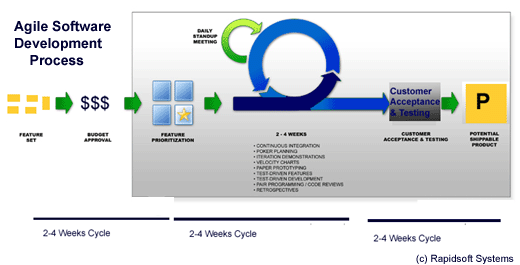
\includegraphics[width=130mm]{./img/development_model.png}
\caption{Agile development model}
\label{fig:development_model}
\end{figure}

By developing iterative and incrementally, the group combined the best from
both the agile development world and from the very well defined waterfall
approach \cite{waterfall}. Feedback from Avdeling BKI and the project mentor has
been very important in the course of the project, in addition to having a
structured and reasonable way of actually doing changes to the plan while the
project was running. At the same time the group was able to maintain the
overall plan within cycles, so that it was possible to work individually, while
still being well coordinated.

To be able to develop all the modules of the project within the timeframe, each
development cycle consisted of multiple modules or functionality developed in
parallel. This allowed for good utilization of time and personnel. The start of
each cycle consisted of a meeting where the goals for the cycle were defined and
individual tasks that we needed to get done were identified. This process bears
similarity to the start of a sprint in the development model Scrum \cite{scrum}.
During the development part of the cycle, the group worked individually on the
tasks that were defined in the planning phase. Regular meetings and cooperative
programming within the group ensured that everyone pulled the project in the
same direction. At the end of each cycle a working set of software was ready,
which ideally complied with all the goals set in the start of each cycle.
Meetings with Avdeling BKI were held between each cycle to present the progress,
and to let them influence the direction of the project.

When all the development cycles were completed, final assurances were made that
everything worked as intended and that all modules coexisted in harmony. This
part of the development also consisted of some hands-on testing by Avdeling BKI
and performance testing.

\subsection{Schedule}
This project had a fairly comprehensive initial phase for mapping
and designing of the system. The group spent the better part of the first two
weeks figuring out how to implement the system. After the two weeks and before
the start of the development, a ``project decision meeting" was held with
Avdeling BKI to get feedback on the design and confirm that the system was
modelled correctly for their needs.

After this, the implementation phase commenced, which consisted of development
cycles as described above in section \ref{sec:dev_method}. This phase was devided into
five parts: four development cycles and a final cleanup/testing cycle. All the
development cycles lasted two weeks, aside from the last development cycle and the cleanup/testing
cycle, which lasted one week each. During these cycles the group conducted
meetings with both the project mentor and Avdeling BKI every two weeks, timed so
that these meetings took place on alternating weeks. This ensured continual
feedback and advice throughout the development process.

After the development phase, focus was shifted from the software to the project
report, and the group spent the final 5-6 weeks working on the report. The group
benefitted from the work performed during the first weeks of the project which
could go almost directly into the report.

\subsection{Project Organization}
The organisation of the project shifted throughout the project, reflecting
the fact that the project had multiple phases. During the first few weeks
the group spent most of the time together in a group room, cooperating in
forming the design and discussing various solutions. Once most things had been
worked out and the implementation phase began, there was more room and need to
work individually to produce code. In this period, the group gathered
together a few times a week to syncronize the progress and plan the next course
of action. Throughout the project, most decisions have been made either by
confering with the client or achieving consensus within the group. 

\section{Document Structure}
TBC: How have we organized this document.

\subsection{Special Styles Used}
Software names are written in a different font throughout the
report, like so: \snowman{}. Source code is listed in an enclosed box with
syntax highlighting (listing \ref{lst:example}). Source code can also appear in
the text with the same syntax highlighting as the listings, especially note
classnames which will appear as so: \pythoninline{ClassName}.

\begin{python}[caption=Source code example.,label=lst:example]
def printHello():
  # Print a message
  print 'Hello World!'
\end{python}